% This file was created by tikzplotlib vunknown.
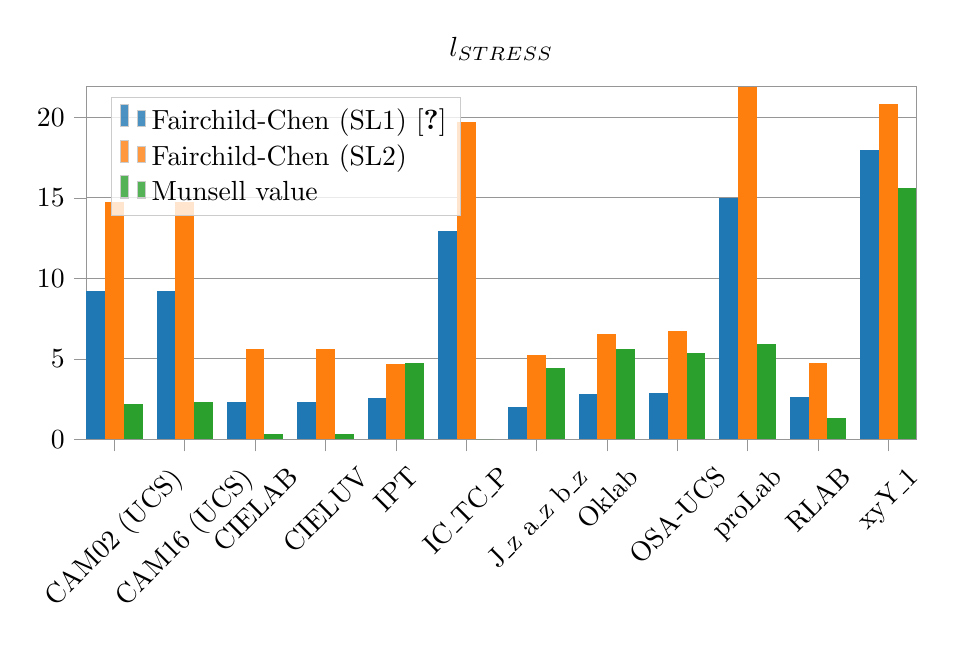
\begin{tikzpicture}

\definecolor{color0}{rgb}{0.12156862745098,0.466666666666667,0.705882352941177}
\definecolor{color1}{rgb}{1,0.498039215686275,0.0549019607843137}
\definecolor{color2}{rgb}{0.172549019607843,0.627450980392157,0.172549019607843}

\begin{axis}[
axis line style={white!58.8235294117647!black},
height=0.5\textwidth,
legend cell align={left},
legend style={fill opacity=0.8, draw opacity=1, text opacity=1, at={(0.03,0.97)}, anchor=north west, draw=white!80!black},
tick align=outside,
tick pos=left,
width=\textwidth,
x grid style={white!58.8235294117647!black},
xmin=-0.4, xmax=11.4,
xtick style={color=white!58.8235294117647!black},
xtick={0,1,2,3,4,5,6,7,8,9,10,11},
xticklabel style = {rotate=45.0},
xticklabels={CAM02 (UCS),CAM16 (UCS),CIELAB,CIELUV,IPT,IC\_TC\_P,J\_z a\_z b\_z,Oklab,OSA-UCS,proLab,RLAB,xyY\_1},
y grid style={white!58.8235294117647!black},
title={$l_\text{STRESS}$},
ymajorgrids,
ymin=0, ymax=43.8017682909425,
ytick style={color=white!58.8235294117647!black},
ytick={0,10,20,30,40,50},
yticklabels={0,5,10,15,20,25}
]
\draw[draw=none,fill=color0] (axis cs:-0.4,0) rectangle (axis cs:-0.133333333333333,18.4645911268359);
\addlegendimage{ybar,ybar legend,draw=none,fill=color0};
\addlegendentry{Fairchild-Chen (SL1) \cite{fairchildchen}}

\draw[draw=none,fill=color0] (axis cs:0.6,0) rectangle (axis cs:0.866666666666667,18.462147583011);
\draw[draw=none,fill=color0] (axis cs:1.6,0) rectangle (axis cs:1.86666666666667,4.67289145504149);
\draw[draw=none,fill=color0] (axis cs:2.6,0) rectangle (axis cs:2.86666666666667,4.67289145504149);
\draw[draw=none,fill=color0] (axis cs:3.6,0) rectangle (axis cs:3.86666666666667,5.16507600277125);
\draw[draw=none,fill=color0] (axis cs:4.6,0) rectangle (axis cs:4.86666666666667,25.8971077549113);
\draw[draw=none,fill=color0] (axis cs:5.6,0) rectangle (axis cs:5.86666666666667,4.0793287828234);
\draw[draw=none,fill=color0] (axis cs:6.6,0) rectangle (axis cs:6.86666666666667,5.64665508676546);
\draw[draw=none,fill=color0] (axis cs:7.6,0) rectangle (axis cs:7.86666666666667,5.82738652177515);
\draw[draw=none,fill=color0] (axis cs:8.6,0) rectangle (axis cs:8.86666666666667,29.9517645366911);
\draw[draw=none,fill=color0] (axis cs:9.6,0) rectangle (axis cs:9.86666666666667,5.27750425239979);
\draw[draw=none,fill=color0] (axis cs:10.6,0) rectangle (axis cs:10.8666666666667,35.9945312574285);
\draw[draw=none,fill=color1] (axis cs:-0.133333333333333,0) rectangle (axis cs:0.133333333333333,29.5046968567554);
\addlegendimage{ybar,ybar legend,draw=none,fill=color1};
\addlegendentry{Fairchild-Chen (SL2)}

\draw[draw=none,fill=color1] (axis cs:0.866666666666667,0) rectangle (axis cs:1.13333333333333,29.4786529029533);
\draw[draw=none,fill=color1] (axis cs:1.86666666666667,0) rectangle (axis cs:2.13333333333333,11.2665102417932);
\draw[draw=none,fill=color1] (axis cs:2.86666666666667,0) rectangle (axis cs:3.13333333333333,11.2665102417932);
\draw[draw=none,fill=color1] (axis cs:3.86666666666667,0) rectangle (axis cs:4.13333333333333,9.42833864558851);
\draw[draw=none,fill=color1] (axis cs:4.86666666666667,0) rectangle (axis cs:5.13333333333333,39.3604065141249);
\draw[draw=none,fill=color1] (axis cs:5.86666666666667,0) rectangle (axis cs:6.13333333333333,10.428911813808);
\draw[draw=none,fill=color1] (axis cs:6.86666666666667,0) rectangle (axis cs:7.13333333333333,13.1227691380623);
\draw[draw=none,fill=color1] (axis cs:7.86666666666667,0) rectangle (axis cs:8.13333333333333,13.4430812029788);
\draw[draw=none,fill=color1] (axis cs:8.86666666666667,0) rectangle (axis cs:9.13333333333333,43.8017682909425);
\draw[draw=none,fill=color1] (axis cs:9.86666666666667,0) rectangle (axis cs:10.1333333333333,9.44336537734861);
\draw[draw=none,fill=color1] (axis cs:10.8666666666667,0) rectangle (axis cs:11.1333333333333,41.6824228979887);
\draw[draw=none,fill=color2] (axis cs:0.133333333333333,0) rectangle (axis cs:0.4,4.37071391926707);
\addlegendimage{ybar,ybar legend,draw=none,fill=color2};
\addlegendentry{Munsell value}

\draw[draw=none,fill=color2] (axis cs:1.13333333333333,0) rectangle (axis cs:1.4,4.60456291212743);
\draw[draw=none,fill=color2] (axis cs:2.13333333333333,0) rectangle (axis cs:2.4,0.692826553107365);
\draw[draw=none,fill=color2] (axis cs:3.13333333333333,0) rectangle (axis cs:3.4,0.692826553107365);
\draw[draw=none,fill=color2] (axis cs:4.13333333333333,0) rectangle (axis cs:4.4,9.47504412245566);
\draw[draw=none,fill=color2] (axis cs:5.13333333333333,0) rectangle (axis cs:5.4,0.0);
\draw[draw=none,fill=color2] (axis cs:6.13333333333333,0) rectangle (axis cs:6.4,8.90523847167804);
\draw[draw=none,fill=color2] (axis cs:7.13333333333333,0) rectangle (axis cs:7.4,11.1924669875584);
\draw[draw=none,fill=color2] (axis cs:8.13333333333333,0) rectangle (axis cs:8.4,10.7060560056212);
\draw[draw=none,fill=color2] (axis cs:9.13333333333333,0) rectangle (axis cs:9.4,11.8658974288993);
\draw[draw=none,fill=color2] (axis cs:10.1333333333333,0) rectangle (axis cs:10.4,2.72811280229079);
\draw[draw=none,fill=color2] (axis cs:11.1333333333333,0) rectangle (axis cs:11.4,31.2517455700297);
\end{axis}

\end{tikzpicture}
